\section{Implementation: First Stage} % 2383bf9c9b47d4ef43480dfd263502892753236d

\subsection{Development}
    \subsubsection{Setting Up Git}
        By nature of using Git for version control, the first step to beginning the project is to create a \texttt{.gitignore} file:

        \inputminted{html}{code/initial/.gitignore}

        Now the project folder can be initialised as a git repository:

        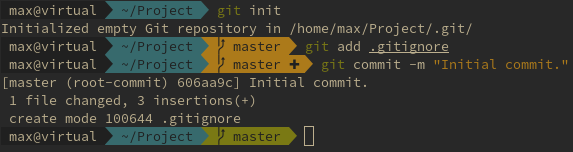
\includegraphics[scale=0.6]{git-setup}

        As mentioned in the Design section, the project code is split into two primary directories: \texttt{include/} and \texttt{src/} with header files stored in the former and source/implementation files in the latter. Inside both of those directories are directories both called \texttt{common}. It is in those directories where the general emulator code is kept (i.e. code not specific to the GUI, testing or CLI).

    \subsubsection{Primitives}

        The first step taken in beginning the actual implementation was to define a collection of primitive types. This was done for a number of reasons. Firstly, the typical built-in types provided in C++ (e.g. \texttt{unsigned int}) have a size that is dependent on the target system and compiler used. The standard library header \texttt{cstdint} provides types such as \texttt{uint16\_t} which are of a definite size (unsigned 16-bit integer in the case of the aforementioned). The issue with these however is that, depending on the compiler, they may be found under the \texttt{std::} namespace only or also in the global namespace. In ensure compatibility across all compilers, one would have to use these types with the \texttt{std::} prefix or make use of the \texttt{using namespace} command for each type they wish to use (so that they are guaranteed to be in the global namespace).

        To resolve this issue, as an alternative to making use of the aforementioned 'using' command, I decided to create type aliases for each of these primitive types with their \texttt{std::} namespace prefix specified. This also allowed me to give cleaner names without the \texttt{\_t} extension in order to aid readability.

        The code of the \texttt{primitives.hpp} header is found in the \texttt{include/common/} directory and is shown below:

        \inputminted{c++}{code/initial/primitives.hpp}

    \subsubsection{Memory}

        An element of the C++ compilation system is that it is advantageous in terms of compile time to keep the declaration of class separate from the implementation of any of its member functions. Class declarations are defined in header files (\texttt{.cpp}) while class implementations are defined in source files (\texttt{.hpp}). In the case of class templates however, the compiler does not allow the implementation to be kept separate from the declaration. This is seen in the \texttt{Memory} class template that follows:

        \inputminted{c++}{code/initial/memory.hpp}

        It was decided that this would indeed be a class template simply to make the code as generic as possible. Should, in some later stage of development, be decided that the values stored in memory or memory addresses would be a different numerical type, the use of this class template makes that an easy change to make.

        There is an exception class that derives from \texttt{std::exception} defined within the \texttt{Memory} class template. Nesting these classes was done so that the exception class could have a member that is the correct type to hold the out-of-bounds address that caused the exception to be thrown.

        The memory values themselves are stored as a raw array, the size of which is not known at compile-time (meaning it has to be dynamically-allocated). This is array is kept within a \texttt{std::unique\_ptr} so that memory will be deallocated automatically when no longer needed. The pointer to this array is declared as private meaning it can only be used within the class itself. This class makes use of encapsulation in the sense that only methods that indirectly modify the internal data can be used from the outside. This has the advantage of ensuring safety as it means users of the class cannot tamper with memory or cause issues by providing invalid values (e.g. attempting to write a value to memory beyond the amount allocated).

        In terms of the public interface, methods for reading from and writing to memory are provided as well as the methods to check whether a given address is within memory bounds or to fill/clear all memory values.

    \subsubsection{CPU} \label{sec:initial-cpu}
        Next, design of the general Intel 8086 class began:

        \inputminted{c++}{code/initial/intel8086.hpp}

        This began with defining some type aliases to make it more explicit what a value's purpose exactly is. For example, it isn't immediately obvious why the \texttt{resolveAddress} method returns an unsigned 32-bit integer, so having it return such a type under the alias \texttt{AbsAddr} indicates that it is returning an absolute memory address and therefore reduces ambiguity.

        Completing fetch-decode-execute cycle with this class design requires a few steps:
        \begin{enumerate}
            \item Fetching the address of the next instruction (i.e. instruction pointer segmented within the code segment) by calling the \texttt{nextInstructionAddress} method.
            \item Passing that address and a \texttt{Memory} object to the \texttt{fetchDecodeInstruction} method which will return the decoded instruction at that address as an object inheriting from the \texttt{Instruction} (and stored within a \texttt{std::unique\_ptr}).
            \item The \texttt{Instruction}-derrived object can then be passed to \texttt{executeInstruction} where it is finally executed.
        \end{enumerate}
        This provides a fair degree of flexibility - the separation of decoding and executing gives the freedom to decode an instruction at a given address (so that its assembly representation may be seen, for example) without then being forced to execute it.

        At this stage in development, the \texttt{Intel8086} class is only declared in a header and is not yet implemented.
        
    \subsubsection{Register Indexes}
        You may have noticed that the CPU class outlined in section \ref{sec:initial-cpu} has register members which are to be declared now. However, before the class templates for the registers themselves are defined, I begin with creating the \texttt{RegisterIndex} class:

        \inputminted{c++}{code/initial/registerindexes.hpp}

        This \texttt{RegisterIndexes} class is to function somewhat like the type of \texttt{enum} one can define in Java - in other words, an enumeration but with additional properties also stored. In this instance, those 'additional properties' are the assembly identifiers and brief descriptions of each register. This class functions like a enumeration by having its constructor be protected and then each enumeration value defined as a static constant member of that class.

        In the above header, indexes for each of general-purpose and segment registers of the Intel 8086 are declared.

        The implementation of this class is fairly simple also:

        \inputminted{c++}{code/initial/registerindexes.cpp}

    \subsubsection{Registers}
        Registers are also represented using class templates so that the aforementioned \texttt{RegisterIndex} may be specified as type arguments - the size of an individual register can also be specified by providing the appropriate type.

        \inputminted{c++}{code/initial/registers.hpp}

        Internally, registers are stored using \texttt{std::map} which maps a \texttt{RegisterIndex} to a register's value. The \texttt{RegistersLowHigh} class makes use of helper functions \texttt{getHighByte} and \texttt{getLowByte} which are outlined in section \ref{sec:initial-helper-functions}.

    \subsubsection{Helper Functions} \label{sec:initial-helper-functions}
        Due to the Intel 8086 having general-purpose registers that can be accessed as individual high or low bytes, it is necessary that the program can extract the most or least significant byte from a 16-bit value. This is what prompted me to create a helper function namespace called \texttt{conversion}.

        \inputminted{c++}{code/initial/conversion.hpp}

        While it currently has only two functions, it is likely that this namespace will become more populated as the project progresses.

        \inputminted{c++}{code/initial/conversion.cpp}

    % TODO: build system bruh.

\subsection{Testing}
    \subsubsection{Testing of Memory} \label{sec:initial-testing-memory}
        The \texttt{Memory} has been fully implemented and is as such ready for proper testing. Below is the unit testing code for this class (using the Catch2 framework):

        \inputminted{c++}{code/initial/testmemory.cpp}

        The results of running these tests:

        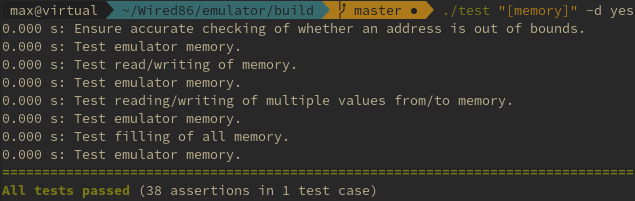
\includegraphics[scale=0.6]{memory-tests}

    \subsubsection{Testing of Helper Functions}
        The two functions of the \texttt{conversion} namespace were also tested.

        \inputminted{c++}{code/initial/testconversions.cpp}

        These tests also all ran successfully.

    \subsubsection{Testing of CPU Registers}
        While the CPU itself is not yet ready to be tested, the CPU register system is complete and therefore ready.

        \inputminted{c++}{code/initial/testregisters.cpp}

        Running these tests shows that the CPU register system devised functions as expected.

\subsection{Review}
    \subsubsection{Overview of Progress}
        After completion of the first stage of development, I now have a working development environment and a codebase that, though it may not yet provide any use to the user, is a solid foundation on which to build. In terms of that foundation, a proper build system with distinctly separate locations for code (common, GUI, CLI, and testing) is provided. For 'common' code, several key emulator components - including the CPU, memory and registers - are now implemented (or at least declared).

    \subsubsection{Success Criteria}
        This first stage of development was able to fully address one emulator success criteria (see table \ref{table:emulator-success-criteria}): \textit{Has emulated memory which can be read and written to by the emulated CPU without error.}

        For evidence that this success criteria was indeed met, please see section \ref{sec:initial-testing-memory}. In said section, one can see that all unit tests designed to ensure emulator memory functions correctly run successfully.

    \subsubsection{Plans}
        There are a few key areas of software that should be addressed next. To begin with, I believe that the software would benefit greatly from some form of proper logging system as currently output is just written to standard out without any form of colour coding, time-stamping, or other such information. In addition, the \texttt{Intel8086} class needs to be implemented. After which I can begin the difficult task of devising a system which can decode the complex x86 instruction set.



\section{Implementation: Second Stage} % ad9b8e1c0d996710b102058cbae76fa0dc8b4745

\subsection{Development}
    \subsubsection{Logging}
        To begin the second stage of development, it was decide that a proper, flexible logging system was integral to for clearly providing information regarding the status of emulator (at least, before the GUI is implemented). I decided that an object-orientated approach would be most appropriate as multiple instance of a \texttt{Logger} class can be created for each logger type (e.g. general information, error, warning, etc.)

        Aside from the colour-coding and time-stamping one would expect from such a system, additional information can be provided to logging output via the \texttt{ADDITIONAL\_LOGGING\_INFO} macro and the \texttt{LoggingInfo} structure. Through the use of the former as the final argument to a logging call, I can have that logging message include information about from where in the code it was called from (line number, file, and from what function).

        The logging system is also not hard-coded to output via standard console output. Instead, it makes use of the C++ standard library's \texttt{std::ostream} object to allow output via any stream (console output, to a file, or even over a network). This is beneficial as it allows logging output to be redirected to a file for later analysis with very little extra effort.

        \inputminted{c++}{code/second/logging.hpp}

        \inputminted{c++}{code/second/logging.cpp}

    \subsubsection{Instruction Opcodes} \label{sec:second-opcodes}
        Finally, it was time to begin the complex task of creating a system capable of representing the complex instruction encoding used by the Intel 8086 CPU. The first step here was to create a class to represent instruction opcodes.

        \inputminted{c++}{code/second/opcode.hpp}

        Aside from of course indicating which operation an instruction will carry out, the opcode of an instruction also indicates (where applicable) whether the instruction operates on byte values or 16-bit values, as well as the 'direction' of the instruction (whether the REG component of the instruction's MOD-REG-R/M byte is acting as a source or destination for the operation). In the \texttt{Opcode} class header above, it can be seen that these are represented using human-readable enumerations \texttt{DataSize} and \texttt{RegDirection} as an alternative to the bit values they are actually stored as.

        \inputminted{c++}{code/second/opcode.cpp}

    \subsubsection{Changes to CPU}
        In the first stage of development, a class by the name of \texttt{Intel8086} was declared. At this second stage, that class is partially implemented:

        \inputminted{c++}{code/second/intel8086.cpp}

    \subsubsection{Conversion/Helper Functions}
        Aside from the \texttt{conversion} namespace being renamed to just \texttt{convert}, a few additional helper functions and function templates were introduced into said namespace. For example, in section \ref{sec:second-opcodes} you will see the use of templates by the name of \texttt{getBitFrom} and \texttt{getBitsFrom} respectively. As their names would imply, these template functions allow for fetching specific bits contained in a value from a given 'index'.

        \inputminted{c++}{code/second/convert.hpp}

        In addition, the function \texttt{createWordFromBytes} was also introduced. This function simply combines a low and high byte in order to produce a resulting 16-bit value.

        \inputminted{c++}{code/second/convert.cpp}

\subsection{Testing}

    \subsubsection{Testing of New Helper/Conversion Code}
        In this second stage of development, additional code was introduced into the \texttt{convert} namespace. Naturally, to ensure the stability of the program, said code should be tested.

        \inputminted{c++}{code/second/furthertestconversions.cpp}

        The above code shows the new unit tests added to the pre-existing section wherein the code of the \texttt{covert} namespace is checked. It was by running these new unit tests that I realised the original implementation of the \texttt{getBitsFrom} function template did not work as I had intended:

        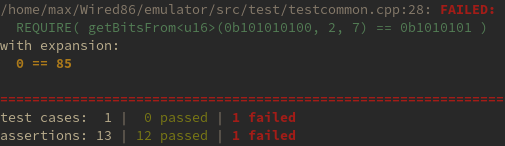
\includegraphics[scale=0.6]{failed-test}

        The above image shows the output when the tests were run and one failed. From this I was able to identify the \texttt{getBitsFrom} function template as containing the faulty code. Upon investigation, I realised the following line had an off-by-one-error: \mint{c++}{T mask = 1 << count;}

        This was causing issues as creating an appropriate bit-mask requires raising 2 to the power of the number of bits and then taking away one. As such, the code was easily corrected: \mint{c++}{T mask = (1 << count) - 1; // (2 ^ count) - 1}


    \subsubsection{Testing of Basic Instruction Representation}
        In terms of CPU instructions, only the \texttt{Opcode} class is fully-implemented at this stage in development.

        \inputminted{c++}{code/second/testinstructions.cpp}

        All these tests ran successfully.

\subsection{Review}
    \subsubsection{Overview of Progress}
        The second stage of development began with the implementation of a more robust logging system which should help with the diagnosis of issues with as well as the general usage of the emulator. In addition the first step towards full instruction decoding was made with the introduction of opcode representation and further improvements to the CPU code.

    \subsubsection{Success Criteria}
        While it does not yet meet it, this stage of development brought the project closer to fulfilling the following success criteria (see table \ref{table:emulator-success-criteria}): \textit{Capable of executing all instructions listed in appendix section 10 successfully including cases where those instructions may include MOD-REG-R/M, immediate and/or displacement bytes.}

        To elaborate, the introduction of the \texttt{Opcode} class is the first key step to meeting the above criteria - said class has been implemented and tested.

    \subsubsection{Plan}
        As for the following stage of development, completing the instruction representation system is a key priority.



\section{Implementation: Third Stage}
